% ============================================================================
%  S3 Maude Module Documentation
%  Maude-HCS  —  S3_AUX  &  S3_PROTOCOL
%  Auto-generated 2026-04-17
% ============================================================================
\documentclass[11pt]{article}

\usepackage[margin=0.9in]{geometry}
\usepackage{listings}
\usepackage{xcolor}
\usepackage{booktabs}
\usepackage{longtable}
\usepackage{array}
\usepackage{hyperref}
\usepackage{amsmath,amssymb}
\usepackage{tikz}
\usetikzlibrary{arrows.meta,positioning,fit,calc}

% Allow line breaks in monospace text at hyphens
\newcommand{\ttt}[1]{\texttt{\hyphenchar\font=`\-\relax #1}}

% ---- Maude listing style ---------------------------------------------------
\lstdefinelanguage{Maude}{
  morekeywords={mod,endm,pr,sort,subsort,op,ops,eq,ceq,rl,crl,if,sload,
                ctor,assoc,comm,id,owise,vars,var,set,rew,print},
  sensitive=true,
  morecomment=[l]{---},
  morestring=[b]",
  literate={=>}{$\Rightarrow$}2 {->}{$\rightarrow$}2 {;;}{$\mathbin{;;}$}2,
}
\lstset{
  language=Maude,
  basicstyle=\ttfamily\small,
  keywordstyle=\bfseries\color{blue!70!black},
  commentstyle=\itshape\color{gray},
  stringstyle=\color{red!70!black},
  breaklines=true,
  frame=single,
  framerule=0.4pt,
  xleftmargin=1em,
  numbers=left,
  numberstyle=\tiny\color{gray},
  numbersep=6pt,
  captionpos=b,
}

\title{\textbf{Maude-HCS S3 Module Documentation}\\[4pt]
       \large\texttt{S3\_AUX} \quad\&\quad \texttt{S3\_PROTOCOL}}
\author{Maude-HCS Project}
\date{April 2026}

\begin{document}
\maketitle
\tableofcontents
\newpage

% ============================================================================
\section{Overview}
% ============================================================================

The S3 modules provide a high-fidelity, actor-based Maude model of the
Amazon~S3 object-storage protocol.  The model is split into two layers:

\begin{description}
  \item[\texttt{S3\_AUX}]  Auxiliary data types: HTTP message constructors,
    header lists, and the server-side in-memory data map.
  \item[\texttt{S3\_PROTOCOL}]  Behavioral rewrite rules for two actor types
    --- the \emph{SDK Client} and the \emph{AWS S3 HTTP Server} --- that
    together implement the full request/response lifecycle including the
    HTTP \texttt{Expect: 100-continue} streaming handshake.
\end{description}

\noindent
Both modules depend on the common Maude-HCS actor infrastructure
(\texttt{CP2\_SORTS}) and the Skyhook auxiliary definitions
(\texttt{SKYHOOK\_AUX}), which supply the abstract S3 request/response
message sorts consumed by upper-layer Skyhook application logic.

\begin{figure}[h]
\centering
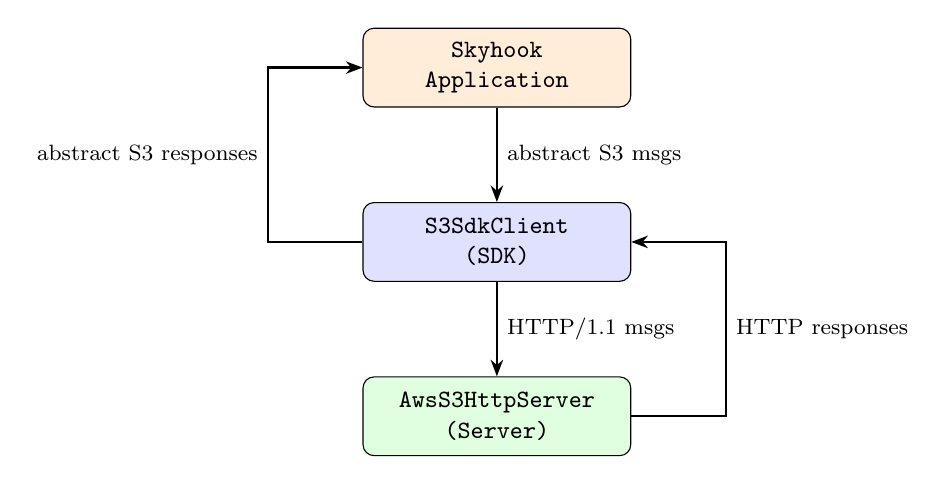
\begin{tikzpicture}[
    box/.style={draw, rounded corners, minimum width=3.4cm,
                minimum height=1cm, align=center, font=\small\ttfamily},
    arr/.style={-{Stealth[length=6pt]}, thick},
  ]
  \node[box, fill=orange!15]  (app) {Skyhook\\Application};
  \node[box, fill=blue!12, below=1.2cm of app] (sdk) {S3SdkClient\\(SDK)};
  \node[box, fill=green!12, below=1.2cm of sdk] (srv) {AwsS3HttpServer\\(Server)};

  \draw[arr] (app.south) -- node[right,font=\footnotesize]{abstract S3 msgs}
             (sdk.north);
  \draw[arr] (sdk.south) -- node[right,font=\footnotesize]{HTTP/1.1 msgs}
             (srv.north);
  \draw[arr] (srv.east)  -- ++(1.2,0) |- node[near start,right,font=\footnotesize]
             {HTTP responses} (sdk.east);
  \draw[arr] (sdk.west)  -- ++(-1.2,0) |- node[near start,left,font=\footnotesize]
             {abstract S3 responses} (app.west);
\end{tikzpicture}
\caption{Layered message flow between Skyhook, SDK Client, and S3 Server.}
\label{fig:arch}
\end{figure}

% ============================================================================
\section{Module \texttt{S3\_AUX}}
\label{sec:s3aux}
% ============================================================================

\subsection{Imported Modules}

\begin{itemize}
  \item \texttt{CP2\_SORTS} --- core Maude-HCS actor sorts
        (\texttt{Actor}, \texttt{Address}, \texttt{Content},
        \texttt{Attribute}, \texttt{AttributeSet}, \texttt{ActorType}).
  \item \texttt{CONVERSION} --- built-in Maude string/number conversion.
  \item \texttt{SKYHOOK\_AUX} --- abstract S3 message sorts
        (\texttt{S3PutObjReq}, \texttt{S3GetObjReq}, etc.).
\end{itemize}

\subsection{Sorts and Subsorts}

\begin{longtable}{@{}p{3.2cm}p{3cm}p{7.5cm}@{}}
\toprule
\textbf{Sort} & \textbf{Subsort of} & \textbf{Purpose} \\
\midrule
\ttt{HttpMethod}    & \ttt{String} & HTTP method verb (e.g.\ \ttt{"GET"}, \ttt{"PUT"}) \\
\ttt{HttpUri}       & \ttt{String} & Request URI path \\
\ttt{HttpBody}      & \ttt{String} & Message body payload \\
\ttt{Header}        & \ttt{S3HeaderList} & Single key--value header \\
\ttt{S3HeaderList}  & ---             & Associative-commutative list of headers \\
\ttt{S3DataMapEntry}& \ttt{S3DataMap} & Single URI $\rightarrow$ Body mapping \\
\ttt{S3DataMap}     & ---             & Associative-commutative map of entries \\
\bottomrule
\end{longtable}

\subsection{Operations}

\subsubsection{Header Construction}

\begin{lstlisting}[caption={Header and header-list operators.}]
op header : String String -> Header [ctor] .
op emptyS3Headers : -> S3HeaderList [ctor] .
op _;;_ : S3HeaderList S3HeaderList -> S3HeaderList
          [ctor assoc comm id: emptyS3Headers] .
\end{lstlisting}

Headers are constructed via \texttt{header(key, value)}.  The \texttt{\_;;\_}
operator merges headers into an unordered, associative-commutative list with
\texttt{emptyS3Headers} as identity, reflecting the fact that HTTP header
ordering is semantically insignificant.

\subsubsection{HTTP Message Constructors}

\begin{longtable}{@{}p{5.8cm}p{8.2cm}@{}}
\toprule
\textbf{Operator} & \textbf{Description} \\
\midrule
{\small\ttt{HttpS3Req(Method, URI, Version, Headers, Body)}}
  & An outgoing HTTP request message sent from the SDK to the server.
    Carries the full set of headers; body may be empty for the initial
    \ttt{Expect: 100-continue} phase. \\[4pt]
{\small\ttt{HttpS3ReqBody(URI, ID, Body)}}
  & A follow-up body-only message, sent after the server acknowledges
    with \ttt{100 Continue}.  Carries the request ID for correlation. \\[4pt]
{\small\ttt{HttpS3Res(StatusCode, Version, Headers, Body)}}
  & An HTTP response from the server.  Status codes used:
    \ttt{100} (Continue), \ttt{200} (OK), \ttt{204} (No Content),
    \ttt{404} (Not Found). \\
\bottomrule
\end{longtable}

\subsubsection{Server Data Map}

\begin{lstlisting}[caption={In-memory server-side object store.}]
op emptyS3DataMap : -> S3DataMap [ctor] .
op _->_ : HttpUri HttpBody -> S3DataMapEntry [ctor] .
op _;_ : S3DataMap S3DataMap -> S3DataMap
         [ctor assoc comm id: emptyS3DataMap] .
\end{lstlisting}

The \texttt{S3DataMap} models the server's in-memory object store as an
associative-commutative set of \texttt{URI $\rightarrow$ Body} entries.

\subsubsection{Map Lookup}

\begin{lstlisting}[caption={Key existence check for the data map.}]
op hasKey : S3DataMap HttpUri -> Bool .
eq hasKey((MAP ; (URI -> BODY)), URI) = true .
eq hasKey(MAP, URI) = false [owise] .
\end{lstlisting}

The \texttt{hasKey} function is used by the server's 404 rule to determine
whether a requested object exists before attempting pattern-matched retrieval.

\subsubsection{Message Sizing}

\begin{lstlisting}[caption={Size equations for network cost modeling.}]
eq getSize(HttpS3Req(M, U, V, H, B)) = 200 .
eq getSize(HttpS3ReqBody(U, ID, B))   = length(B) .
eq getSize(HttpS3Res(S, V, H, B))     = 200 .
\end{lstlisting}

These equations feed the Maude-HCS bandwidth accounting layer.  Request and
response envelopes carry a fixed 200-byte overhead; body-only messages are
sized by payload length.

% ============================================================================
\section{Module \texttt{S3\_PROTOCOL}}
\label{sec:s3protocol}
% ============================================================================

\subsection{Imported Modules}

\begin{itemize}
  \item \texttt{S3\_AUX} (Section~\ref{sec:s3aux})
  \item \texttt{SKYHOOK\_AUX}
\end{itemize}

\subsection{Pending-Request Map}

The SDK client must correlate asynchronous HTTP responses back to the
original abstract S3 request.  This is accomplished with a
\emph{pending-request map}:

\begin{lstlisting}[caption={Pending-request map sorts and operators.}]
sort S3ReqEntry S3ReqMap .
subsort S3ReqEntry < S3ReqMap .
op emptyS3ReqMap : -> S3ReqMap [ctor] .
op _~>_[_] : Nat Content Address -> S3ReqEntry [ctor] .
op _;_ : S3ReqMap S3ReqMap -> S3ReqMap
         [ctor assoc comm id: emptyS3ReqMap] .
\end{lstlisting}

Each entry \texttt{ID \char`\~> OriginalMsg [ CallerAddr ]} records:
\begin{itemize}
  \item \texttt{ID} --- a monotonically increasing request identifier
        (also carried as the \texttt{x-amz-request-id} header),
  \item \texttt{OriginalMsg} --- the abstract S3 message that initiated
        the request,
  \item \texttt{CallerAddr} --- the address to which the abstract response
        must be delivered.
\end{itemize}

\subsection{Actor Types}

\begin{longtable}{@{}p{3cm}p{4.2cm}p{6.5cm}@{}}
\toprule
\textbf{Actor Type} & \textbf{Attributes} & \textbf{Role} \\
\midrule
\ttt{S3SdkClient}
  & {\small\ttt{realAwsAddr}, \ttt{pendingReqs}, \ttt{nextId}, \ttt{thisAddr}}
  & Translates abstract S3 messages into HTTP requests and correlates
    asynchronous HTTP responses back to the originating caller. \\[4pt]
\ttt{AwsS3HttpServer}
  & {\small\ttt{s3DataMap}, \ttt{thisAddr}}
  & Serves HTTP requests, maintains an in-memory object store, and
    implements the \ttt{100-continue} handshake. \\
\bottomrule
\end{longtable}

% ----------------------------------------------------------------------------
\subsection{SDK Client Rules --- Outbound (Abstract $\rightarrow$ HTTP)}
\label{sec:sdk-out}
% ----------------------------------------------------------------------------

Each outbound rule translates an abstract S3 message into a well-formed
\texttt{HttpS3Req}, registers the pending request, and increments the ID
counter.

\begin{longtable}{@{}p{4.5cm}p{1.6cm}p{7.5cm}@{}}
\toprule
\textbf{Rule Label} & \textbf{Method} & \textbf{Behavior} \\
\midrule
{\small\ttt{sdk-put-obj}}
  & \ttt{PUT}
  & Translates \ttt{S3PutObjReq(B,U,D)} into a PUT to
    \ttt{/B/U} with \ttt{Expect: 100-continue}.  Body is deferred. \\[3pt]
{\small\ttt{sdk-get-obj}}
  & \ttt{GET}
  & Translates \ttt{S3GetObjReq(B,U)} into a GET to \ttt{/B/U}.
    No body or continuation header. \\[3pt]
{\small\ttt{sdk-delete-obj}}
  & \ttt{DELETE}
  & Translates \ttt{S3DeleteObjReq(B,U)} into a DELETE to \ttt{/B/U}. \\[3pt]
{\small\ttt{sdk-create-bucket}}
  & \ttt{PUT}
  & Translates \ttt{S3CreateBucketReq(B,R)} into a PUT to \ttt{/B}
    with \ttt{Expect: 100-continue}.  Region XML sent after 100. \\[3pt]
{\small\ttt{sdk-put-policy}}
  & \ttt{PUT}
  & Translates \ttt{S3PutBucketPolicyReq(B,P)} into a PUT to
    \ttt{/B?policy} with continuation. \\[3pt]
{\small\ttt{sdk-put-public-access-block}}
  & \ttt{PUT}
  & Translates \ttt{S3PutPublicAccessBlockReq(B)} into a PUT to
    \ttt{/B?publicAccessBlock} with continuation. \\
\bottomrule
\end{longtable}

% ----------------------------------------------------------------------------
\subsection{SDK Client Rules --- Inbound 100-Continue Handling}
\label{sec:sdk-100}
% ----------------------------------------------------------------------------

When the server responds with \texttt{HttpS3Res(100, \ldots)}, the SDK
matches the \texttt{x-amz-request-id} header against its pending-request map
and transmits the deferred body via \texttt{HttpS3ReqBody}.

\begin{longtable}{@{}p{6.8cm}p{7cm}@{}}
\toprule
\textbf{Rule Label} & \textbf{Body Transmitted} \\
\midrule
{\small\ttt{sdk-handle-100-continue-put-obj}}
  & Raw object data (\ttt{DATA}). \\[3pt]
{\small\ttt{sdk-handle-100-continue-create-\linebreak bucket}}
  & XML with region. \\[3pt]
{\small\ttt{sdk-handle-100-continue-put-policy}}
  & Policy JSON string. \\[3pt]
{\small\ttt{sdk-handle-100-continue-put-\linebreak public-access-block}}
  & XML. \\
\bottomrule
\end{longtable}

All four rules are \emph{conditional} (\texttt{crl}), guarded by the
predicate:
\[
  \texttt{REQ\_ID} == \texttt{string(ID, 10)}
\]
ensuring correct correlation between response and pending request.

% ----------------------------------------------------------------------------
\subsection{SDK Client Rules --- Inbound Final Responses}
\label{sec:sdk-final}
% ----------------------------------------------------------------------------

Upon receiving a terminal HTTP response (200, 204, or 404), the SDK removes
the entry from \texttt{pendingReqs} and delivers the corresponding abstract
S3 response to the original caller.

\begin{longtable}{@{}p{5.2cm}p{1.5cm}p{6.5cm}@{}}
\toprule
\textbf{Rule Label} & \textbf{Status} & \textbf{Abstract Response} \\
\midrule
{\small\ttt{sdk-handle-put-res}}
  & 200
  & \ttt{S3PutObjRes(BUCKET, UUID)} \\[3pt]
{\small\ttt{sdk-handle-get-res}}
  & 200
  & \ttt{S3GetObjRes(BUCKET, UUID, BODY)} \\[3pt]
{\small\ttt{sdk-handle-get-err-res}}
  & 404
  & \ttt{S3GetObjErr(BUCKET, UUID)} \\[3pt]
{\small\ttt{sdk-handle-delete-res}}
  & 204
  & \ttt{S3DeleteObjRes(BUCKET, UUID)} \\[3pt]
{\small\ttt{sdk-handle-create-bucket-res}}
  & 200
  & \ttt{S3CreateBucketRes(BUCKET)} \\[3pt]
{\small\ttt{sdk-handle-put-policy-res}}
  & 200
  & \ttt{S3PutBucketPolicyRes(BUCKET)} \\[3pt]
{\small\ttt{sdk-handle-public-access-\linebreak block-res}}
  & 200
  & \ttt{S3PutPublicAccessBlockRes(BUCKET)} \\
\bottomrule
\end{longtable}

% ----------------------------------------------------------------------------
\subsection{AWS S3 HTTP Server Rules}
\label{sec:server}
% ----------------------------------------------------------------------------

The server actor implements four rules covering the complete object
lifecycle:

\begin{longtable}{@{}p{4.8cm}p{8.8cm}@{}}
\toprule
\textbf{Rule Label} & \textbf{Behavior} \\
\midrule
{\small\ttt{server-handle-put-obj-expect}}
  & Matches any incoming \ttt{PUT} carrying
    \ttt{Expect: 100-continue}.  Responds with
    \ttt{HttpS3Res(100, ...)} to signal readiness for the body.
    \emph{Unconditional rule.} \\[6pt]
{\small\ttt{server-handle-put-obj-data}}
  & Receives the follow-up \ttt{HttpS3ReqBody}.  Inserts the
    URI ${\rightarrow}$ BODY entry into the data map and responds
    \ttt{200 OK}.  \emph{Unconditional rule.} \\[6pt]
{\small\ttt{server-handle-get-obj}}
  & Pattern-matches the requested URI against the data map.
    If found, responds \ttt{200 OK} with the stored body payload.
    \emph{Unconditional rule; the URI must appear in the map for the
    pattern match to succeed.} \\[6pt]
{\small\ttt{server-handle-get-obj-not-found}}
  & Fires when a \ttt{GET} arrives and \ttt{hasKey(DATA\_MAP, URI)}
    is \ttt{false}.  Responds \ttt{404 Not Found} with an empty
    body.  \emph{Conditional rule.} \\[6pt]
{\small\ttt{server-handle-delete-obj}}
  & Pattern-matches the URI in the data map, removes the entry,
    and responds \ttt{204 No Content}.
    \emph{Unconditional rule.} \\
\bottomrule
\end{longtable}

% ============================================================================
\section{Protocol Interaction: Expect 100-Continue Flow}
\label{sec:100continue}
% ============================================================================

The \texttt{PUT}-family operations implement the HTTP/1.1
\texttt{Expect: 100-continue} handshake as a two-phase protocol:

\begin{enumerate}
  \item \textbf{Phase 1 --- Header Exchange.}  The SDK sends an
        \texttt{HttpS3Req} with an empty body and the header
        \texttt{Expect: 100-continue}.  The server responds
        \texttt{HttpS3Res(100, \ldots)}.
  \item \textbf{Phase 2 --- Body Transmission.}  Upon receiving the 100
        response, the SDK transmits the real payload via
        \texttt{HttpS3ReqBody}.  The server absorbs the body, updates its
        data map, and responds \texttt{200~OK}.
\end{enumerate}

\noindent
This two-phase model faithfully captures the real AWS S3 streaming behavior
where large payloads are only transmitted after the server signals readiness.

\begin{figure}[h]
\centering
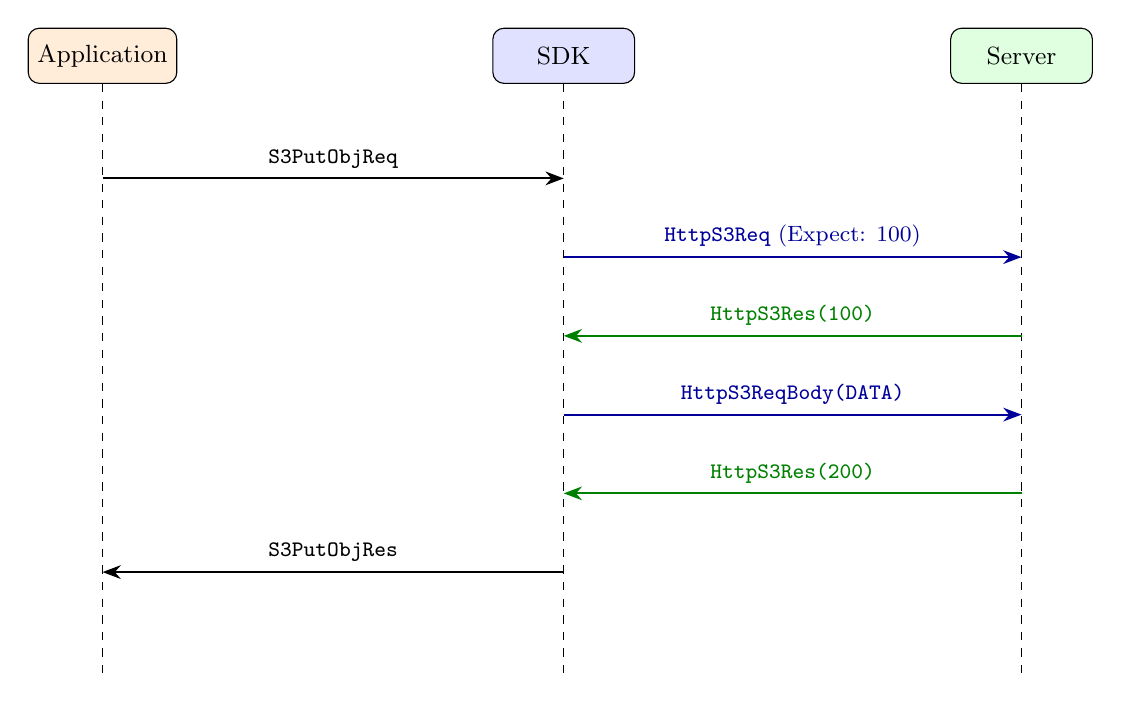
\begin{tikzpicture}[
    node distance=0.6cm,
    every node/.style={font=\small},
    act/.style={draw, minimum width=1.8cm, minimum height=0.7cm,
                rounded corners, fill=#1},
  ]
  % Actors
  \node[act=orange!15] (app) {Application};
  \node[act=blue!12, right=4cm of app] (sdk) {SDK};
  \node[act=green!12, right=4cm of sdk] (srv) {Server};

  % Lifelines
  \draw[dashed] (app.south) -- ++(0,-7.5);
  \draw[dashed] (sdk.south) -- ++(0,-7.5);
  \draw[dashed] (srv.south) -- ++(0,-7.5);

  % Messages
  \draw[-{Stealth},thick] ([yshift=-1.2cm]app.south) --
    node[above,font=\footnotesize]{\texttt{S3PutObjReq}}
    ([yshift=-1.2cm]sdk.south);

  \draw[-{Stealth},thick,blue!60!black] ([yshift=-2.2cm]sdk.south) --
    node[above,font=\footnotesize]{\texttt{HttpS3Req} (Expect: 100)}
    ([yshift=-2.2cm]srv.south);

  \draw[{Stealth}-,thick,green!50!black] ([yshift=-3.2cm]sdk.south) --
    node[above,font=\footnotesize]{\texttt{HttpS3Res(100)}}
    ([yshift=-3.2cm]srv.south);

  \draw[-{Stealth},thick,blue!60!black] ([yshift=-4.2cm]sdk.south) --
    node[above,font=\footnotesize]{\texttt{HttpS3ReqBody(DATA)}}
    ([yshift=-4.2cm]srv.south);

  \draw[{Stealth}-,thick,green!50!black] ([yshift=-5.2cm]sdk.south) --
    node[above,font=\footnotesize]{\texttt{HttpS3Res(200)}}
    ([yshift=-5.2cm]srv.south);

  \draw[{Stealth}-,thick] ([yshift=-6.2cm]app.south) --
    node[above,font=\footnotesize]{\texttt{S3PutObjRes}}
    ([yshift=-6.2cm]sdk.south);
\end{tikzpicture}
\caption{Sequence diagram for a \texttt{PUT} object with \texttt{Expect: 100-continue}.}
\label{fig:seq-put}
\end{figure}

% ============================================================================
\section{Protocol Interaction: GET with 404 Recovery}
\label{sec:404}
% ============================================================================

The \texttt{GET} path supports two outcomes depending on server state:

\begin{itemize}
  \item \textbf{Object exists} --- the server rule
        \texttt{server-handle-get-obj} pattern-matches the URI in the data
        map and returns \texttt{200 OK} with the payload body.  The SDK
        translates this to \texttt{S3GetObjRes}.
  \item \textbf{Object absent} --- the conditional rule
        \texttt{server-handle-get-obj-not-found} fires when
        \texttt{hasKey} returns \texttt{false}, producing
        \texttt{HttpS3Res(404, \ldots)}.  The SDK translates this to
        \texttt{S3GetObjErr}.
\end{itemize}

\noindent
The 404 path enables upper-layer retry logic (e.g.\ the Skyhook
\texttt{ah-handle-incoming-get-err} rule) to detect object absence and
defer fetching until the object has been uploaded.

% ============================================================================
\section{Complete Rule Index}
\label{sec:index}
% ============================================================================

{\small
\begin{longtable}{@{}r p{8cm} l l@{}}
\toprule
\textbf{\#} & \textbf{Rule Label} & \textbf{Type} & \textbf{\S} \\
\midrule
\multicolumn{4}{@{}l}{\emph{SDK Client --- Outbound}} \\
1  & \ttt{sdk-put-obj}               & \ttt{rl}  & \ref{sec:sdk-out} \\
2  & \ttt{sdk-get-obj}               & \ttt{rl}  & \ref{sec:sdk-out} \\
3  & \ttt{sdk-delete-obj}            & \ttt{rl}  & \ref{sec:sdk-out} \\
4  & \ttt{sdk-create-bucket}         & \ttt{rl}  & \ref{sec:sdk-out} \\
5  & \ttt{sdk-put-policy}            & \ttt{rl}  & \ref{sec:sdk-out} \\
6  & \ttt{sdk-put-public-access-block} & \ttt{rl} & \ref{sec:sdk-out} \\
\midrule
\multicolumn{4}{@{}l}{\emph{SDK Client --- 100-Continue}} \\
7  & \ttt{sdk-handle-100-continue-put-obj}   & \ttt{crl} & \ref{sec:sdk-100} \\
8  & \ttt{sdk-handle-100-continue-create-bucket} & \ttt{crl} & \ref{sec:sdk-100} \\
9  & \ttt{sdk-handle-100-continue-put-policy}    & \ttt{crl} & \ref{sec:sdk-100} \\
10 & \ttt{sdk-handle-100-continue-put-public-access-block} & \ttt{crl} & \ref{sec:sdk-100} \\
\midrule
\multicolumn{4}{@{}l}{\emph{SDK Client --- Final Responses}} \\
11 & \ttt{sdk-handle-put-res}        & \ttt{crl} & \ref{sec:sdk-final} \\
12 & \ttt{sdk-handle-get-res}        & \ttt{crl} & \ref{sec:sdk-final} \\
13 & \ttt{sdk-handle-get-err-res}    & \ttt{crl} & \ref{sec:sdk-final} \\
14 & \ttt{sdk-handle-delete-res}     & \ttt{crl} & \ref{sec:sdk-final} \\
15 & \ttt{sdk-handle-create-bucket-res}   & \ttt{crl} & \ref{sec:sdk-final} \\
16 & \ttt{sdk-handle-put-policy-res}      & \ttt{crl} & \ref{sec:sdk-final} \\
17 & \ttt{sdk-handle-public-access-block-res} & \ttt{crl} & \ref{sec:sdk-final} \\
\midrule
\multicolumn{4}{@{}l}{\emph{AWS S3 HTTP Server}} \\
18 & \ttt{server-handle-put-obj-expect}     & \ttt{rl}  & \ref{sec:server} \\
19 & \ttt{server-handle-put-obj-data}       & \ttt{rl}  & \ref{sec:server} \\
20 & \ttt{server-handle-get-obj}            & \ttt{rl}  & \ref{sec:server} \\
21 & \ttt{server-handle-get-obj-not-found}  & \ttt{crl} & \ref{sec:server} \\
22 & \ttt{server-handle-delete-obj}         & \ttt{rl}  & \ref{sec:server} \\
\bottomrule
\end{longtable}
}

\end{document}
